%%%%%%%%%%%%%%%%%%%%%%%%%%%%%%%%%%%%%%%%%%%%%%%%%%%%%%%%%%%%%%%%%%%%%%%%%%%%%%%%%%%%%
%																					%
%	TRABAJO: Proyecto Integrador													%
%																					%
%		Titulo: 	Desarrollo de IP cores con procesamiento de Redes de Petri 		%
%					Temporales para sistemas multicore en FPGA						%
%																					%
%		Autores:	Juli�n Nonino													%
%					Carlos Renzo Pisetta											%
%		Director:	Orlando Micolini												%
%																					%
%	Parte: Resultados y Conclusiones												%
%	Capitulo: Resultados															%
%	Seccion: Interrupciones en el procesador de Redes de Petri						%	
%	Archivo: resultados_interrupciones.tex											%
%																					%
%%%%%%%%%%%%%%%%%%%%%%%%%%%%%%%%%%%%%%%%%%%%%%%%%%%%%%%%%%%%%%%%%%%%%%%%%%%%%%%%%%%%%

% Path Imagenes: ./resultado_conclusiones/resultados/img
% Nombre predeterminado imagenes: resultadosxx
%	xx es el numero de imagen	

\section{Interrupciones en el procesador de Redes de Petri}
	\label{sec:resultados_interrupciones}
	
	El procesador de Redes de Petri, es capaz de generar interrupciones notificando a los hilos/procesos que
	un disparo ha sido ejecutado, por �sta raz�n, en �sta secci�n, presentamos mediciones sobre como afecta
	al rendimiento del sistema el uso de interrupciones en lugar de los otros m�todos de espera.
			
	Para las mediciones, se utiliz� la siguiente Red de Petri (Figura \ref{fig:resultados20}). En dicha Figura, 
	se muestra la red con las diferentes cantidades de tokens en la plaza $P0$. 
			
	\begin{figure}[H]
		\centering
		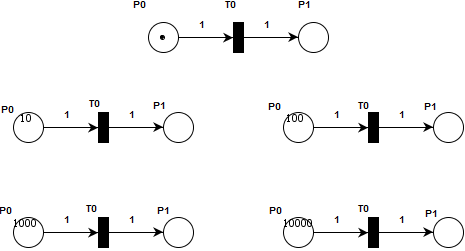
\includegraphics[width=1\linewidth,keepaspectratio]{./resultados_conclusiones/resultados/img/resultados20}
		\caption{Red de Petri utilizada para la medici�n de las interrupciones}
		\label{fig:resultados20}
	\end{figure}
	
	\newpage		
			
	Luego, se se arm� la siguiente tabla con los valores obtenidos.
	
	\begin{figure}[H]
		\centering
		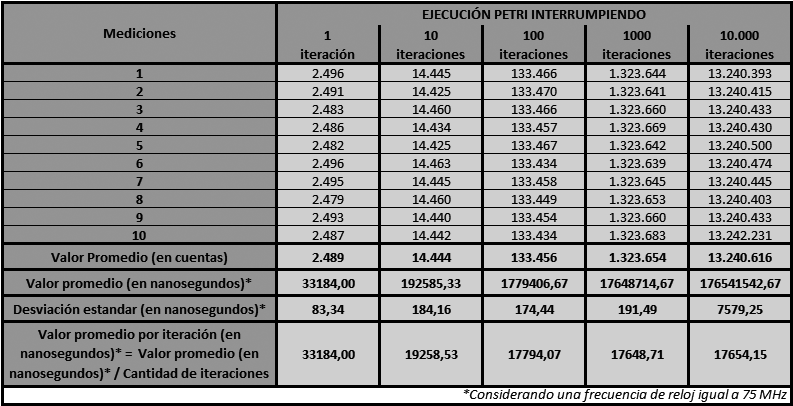
\includegraphics[width=0.9\linewidth,keepaspectratio]{./resultados_conclusiones/resultados/img/resultados21}
		\caption{Tabla de resultados obtenidos utilizando el procesador de Redes de Petri con interrupciones}
		\label{fig:resultados21}
	\end{figure}
	\begin{figure}[H]
		\centering
		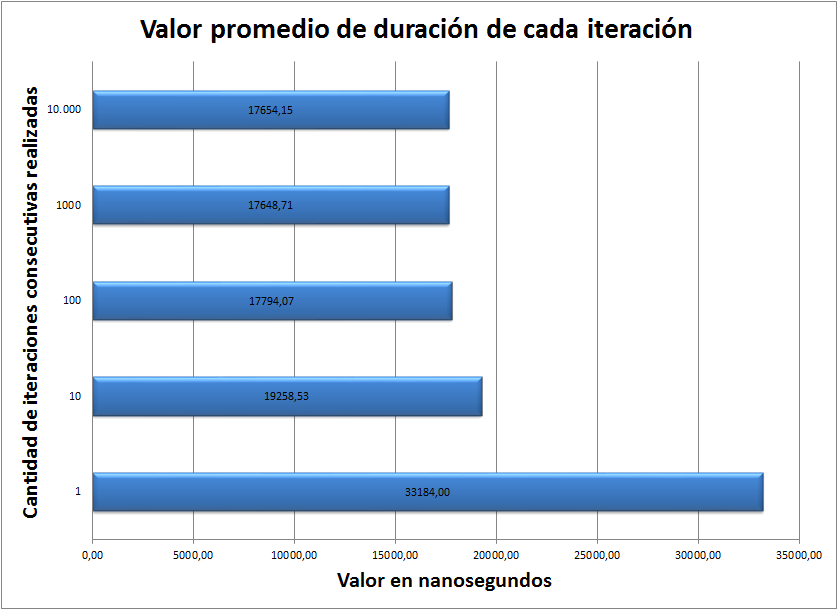
\includegraphics[width=0.9\linewidth,keepaspectratio]{./resultados_conclusiones/resultados/img/resultados22}
		\caption{Valor promedio de duraci�n de cada iteraci�n dependiendo de la cantidad de repeticiones que se realizan en cada ejecuci�n}
		\label{fig:resultados22}
	\end{figure}			
	
	A continuaci�n, se repetir�n las gr�ficas de las Figuras \ref{fig:resultados18} y \ref{fig:resultados19} pero, comparando
	el procesador de Redes de Petri CON y SIN interrupciones.
	
	\begin{figure}[H]
		\centering
		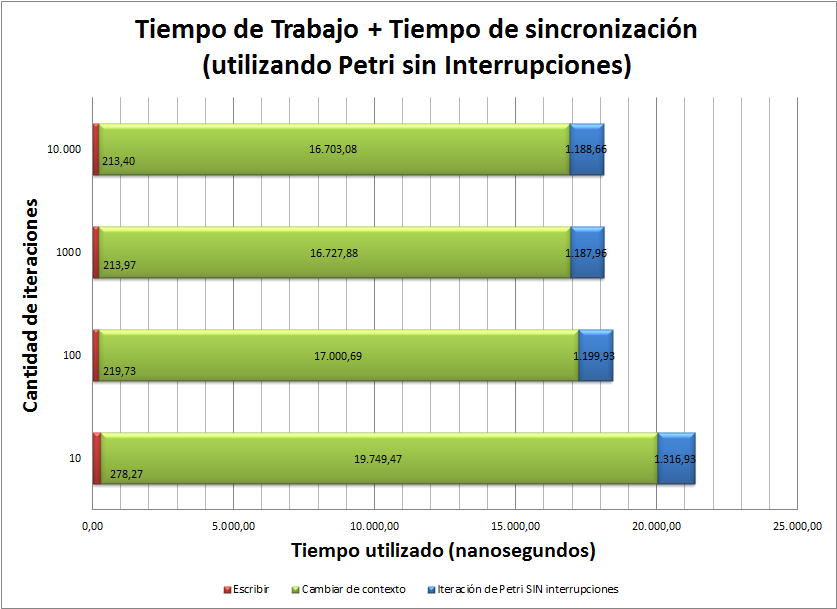
\includegraphics[width=0.8\linewidth,keepaspectratio]{./resultados_conclusiones/resultados/img/resultados23}
		\caption{Carga de trabajo m�s sincronizaci�n utilizando el procesador de Redes de Petri SIN interrupciones}
		\label{fig:resultados23}
	\end{figure}
	\begin{figure}[H]
		\centering
		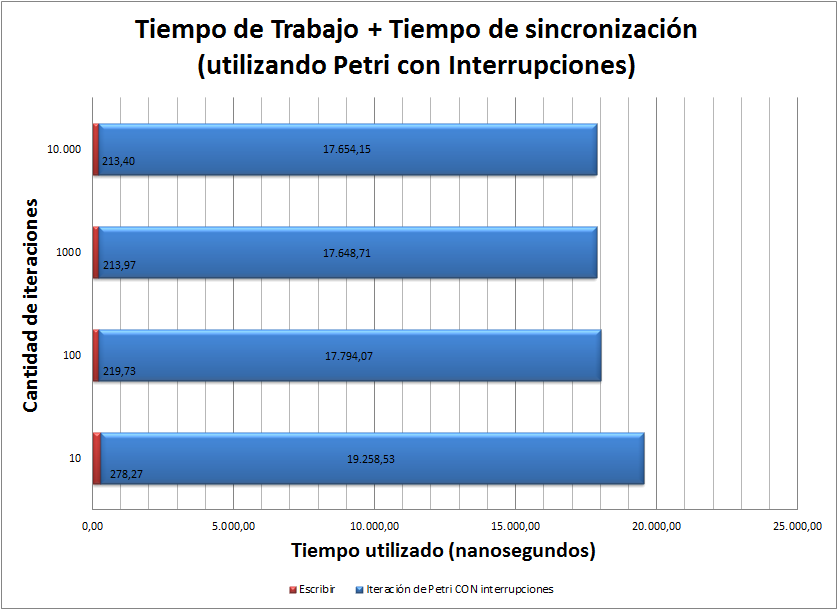
\includegraphics[width=0.8\linewidth,keepaspectratio]{./resultados_conclusiones/resultados/img/resultados24}
		\caption{Carga de trabajo m�s sincronizaci�n utilizando el procesador de Redes de Petri CON interrupciones}
		\label{fig:resultados24}
	\end{figure}
	
	Se debe notar que en la gr�fica con los datos de las interrupciones (Figura \ref{fig:resultados24}) no se incluye
	la duraci�n de un cambio de contexto. �sto se debe a que al utilizar interrupciones, el proceso se suspende siempre
	y se produce un cambio de contexto al llegar la interrupci�n y otro al darle el control nuevamente al hilo, ya reactivado,
	para que siga su funci�n. Por ello, la duraci�n del cambio de contexto est� incluida dentro del tiempo de sincronizaci�n
	consumido por el procesador de Redes de Petri.
	
	En las Figuras \ref{fig:resultados23} y \ref{fig:resultados24} se observa que el uso de interrupciones hace que
	la carga de trabajo de escribir una variable m�s el tiempo de sincronziaci�n sea aproximadamente $1000$ nanosegundos
	menor que sin utilizar interrupciones.
	